\documentclass[border=8pt]{standalone}
% Shared TikZ style for every figure in "Post-training LLMs with RL" (see ../STYLE.md).
% Visual grammar follows the FME office-hours house style; the one accent colour is fern green.
% Compile with XeLaTeX, two passes (annotated equations remember node positions).
\usepackage{fontspec}
\setmainfont{Avenir Next}[BoldFont={Avenir Next Demi Bold}, ItalicFont={Avenir Next Italic}]
\setsansfont{Avenir Next}[BoldFont={Avenir Next Demi Bold}, ItalicFont={Avenir Next Italic}]
\renewcommand{\familydefault}{\sfdefault}
\hyphenpenalty=10000 \exhyphenpenalty=10000 % no hyphenation in notes and labels
\usepackage{amsmath,amssymb}
\usepackage{tikz}
\usetikzlibrary{arrows.meta,positioning,calc,fit,backgrounds,shapes.geometric,decorations.pathreplacing}

% ---------------- palette ----------------
\definecolor{ink}{HTML}{111111}
\definecolor{grey700}{HTML}{4A4F55}
\definecolor{grey500}{HTML}{6B7178}
\definecolor{grey400}{HTML}{8A9097}
\definecolor{grey300}{HTML}{D5D9DD}
\definecolor{grey100}{HTML}{F4F5F6}
\definecolor{fern}{HTML}{4F7942}       % the one accent: what the figure is about
\definecolor{ferndark}{HTML}{2F4A28}
\definecolor{fernlight}{HTML}{B5CFA8}
\definecolor{ferntint}{HTML}{EAF1E6}
% aliases used by older figure files
\colorlet{gray7}{grey700}\colorlet{gray5}{grey500}\colorlet{gray3}{grey300}\colorlet{gray1}{grey100}

% ---------------- visual grammar ----------------
\tikzset{
  every picture/.style={line cap=round, line join=round, color=ink},
  tensor/.style={draw=ink, line width=0.8pt, fill=white},
  param/.style={draw=grey700, line width=0.8pt, fill=grey100},
  op/.style={draw=grey500, line width=0.8pt, rounded corners=3pt, fill=white, inner sep=4pt, font=\small},
  accent/.style={draw=fern, line width=1.2pt},
  flow/.style={-{Stealth[length=5pt]}, line width=0.8pt, draw=grey700},
  flowa/.style={flow, draw=fern},
  tname/.style={font=\normalsize, text=ink},
  dims/.style={font=\footnotesize, text=grey500},
  note/.style={font=\footnotesize, text=grey700, align=left},
  accentnote/.style={font=\footnotesize, text=fern, align=left},
  lead/.style={draw=grey400, line width=0.5pt},
  stream/.style={draw=grey300, line width=5pt},
  block/.style={draw=grey500, line width=0.8pt, rounded corners=4pt, fill=white, align=center, font=\small, minimum height=0.8cm},
  blocka/.style={block, accent, fill=ferntint},
  frozen/.style={block, fill=grey100},
  plus/.style={circle, draw=grey700, line width=0.8pt, fill=white, inner sep=0pt, minimum size=0.42cm, font=\small},
  junction/.style={circle, fill=grey700, inner sep=0pt, minimum size=4pt},
  wire/.style={line width=0.8pt, draw=grey700},
}

% ---------------- numbered annotation system ----------------
%   markers on the drawing:  \mk{(x,y)}{1}   \mka{(x,y)}{2} (accent)
%   notes column:            \notesat{(x,y)}{width}  then  \note{1}{text}  /  \notea{2}{text}
%   symbols strip:           \symbols{$x$ & prompt \\ $y$ & response}
\tikzset{
  marker/.style={circle, fill=grey700, text=white, font=\footnotesize\bfseries, inner sep=0pt, minimum size=0.46cm},
  markera/.style={marker, fill=fern},
}
\newcommand{\mk}[2]{\node[marker] at #1 {#2}}
\newcommand{\mka}[2]{\node[markera] at #1 {#2}}
\newlength{\notewidth}
\newcommand{\notesat}[2]{%
  \node[inner sep=0pt, minimum size=0pt, anchor=north west] (note0) at #1 {};
  \setlength{\notewidth}{#2}\xdef\lastnote{note0}}
\newcommand{\note}[2]{%
  \node[font=\small, text=ink, align=left, text width=\notewidth, anchor=north west, inner sep=0pt] (note#1) at ($(\lastnote.south west)+(0.55cm,-0.32cm)$) {#2};
  \node[marker] at ($(note#1.north west)+(-0.30cm,-0.15cm)$) {#1};
  \path (note#1.south west) ++(-0.55cm,0) node[inner sep=0pt, minimum size=0pt] (note#1base) {};
  \xdef\lastnote{note#1base}}
\newcommand{\notea}[2]{%
  \node[font=\small, text=ferndark, align=left, text width=\notewidth, anchor=north west, inner sep=0pt] (note#1) at ($(\lastnote.south west)+(0.55cm,-0.32cm)$) {#2};
  \node[markera] at ($(note#1.north west)+(-0.30cm,-0.15cm)$) {#1};
  \path (note#1.south west) ++(-0.55cm,0) node[inner sep=0pt, minimum size=0pt] (note#1base) {};
  \xdef\lastnote{note#1base}}
\newcommand{\symbols}[1]{%
  \node[anchor=north west, inner sep=0pt, align=left, font=\small, text=grey700] (symbols)
    at ($(\lastnote.south west)+(0,-0.75cm)$)
    {\textcolor{grey400}{\scriptsize\bfseries SYMBOLS}\\[3pt]
     \begin{tabular}{@{}l@{\hspace{8pt}}l@{}}#1\end{tabular}};
  \draw[grey300, line width=0.5pt] ($(symbols.north west)+(0,0.18cm)$) -- ++(\notewidth+0.55cm,0);}

% ---------------- glyphs ----------------
\tikzset{
  expand/.style={draw=grey700, line width=0.8pt, fill=grey100, trapezium, trapezium stretches body,
                 trapezium left angle=64, trapezium right angle=64, shape border rotate=180,
                 minimum height=0.72cm, align=center, font=\small, inner xsep=2pt},
  contract/.style={expand, shape border rotate=0},
  silubox/.style={block, path picture={
      \begin{scope}[sharp corners, shift={($(path picture bounding box.west)+(0.45,-0.05)$)}, x=0.1cm, y=0.1cm]
        \draw[grey300, line width=0.4pt] (-3,0) -- (2.6,0);
        \draw[grey500, line width=1pt, domain=-3:2.4, samples=30] plot (\x, {\x/(1+exp(-\x))});
      \end{scope}}},
}

% ---------------- annotated equations (arrow + plain-language label per term) ----------------
% \tm{name}{math}: wrap one term of a formula in a named node. Put the formula node at (0,0)
% with anchor=base west, otherwise the remembered positions are offset.
\newcommand{\tm}[2]{\tikz[remember picture,baseline=(#1.base)]{\node[inner sep=1pt,outer sep=0pt] (#1) {$\displaystyle #2$};}}
\tikzset{
  lbl/.style   = {font=\large, text=ferndark, align=left, inner sep=2pt},
  lblg/.style  = {lbl, text=grey700},
  arr/.style   = {-{Stealth[length=8pt,width=6pt]}, line width=1.0pt, draw=fern, shorten >=3pt},
  arrg/.style  = {arr, draw=grey500},
  brc/.style   = {decorate, decoration={brace, mirror, amplitude=9pt, raise=5pt}, line width=1.4pt},
  % older diagram styles (kept for existing figures)
  blk/.style   = {draw=grey500, line width=0.9pt, rounded corners=6pt, fill=white, align=center, inner sep=7pt, minimum height=11mm, text=ink},
  blkf/.style  = {blk, draw=fern, line width=1.2pt, fill=ferntint},
  blkg/.style  = {blk, fill=grey100},
  ar/.style    = {-{Stealth[length=7pt,width=5pt]}, line width=1.0pt, draw=grey700},
  arf/.style   = {ar, draw=fern},
  capt/.style  = {font=\normalsize, text=grey500, align=center},
}

% ---------------- annotation protocol for equations ----------------
% The formula is one node named "eq" at (0,0), anchor=base west. Terms are wrapped with \tm.
% Labels sit in fixed rows ABOVE (a) or BELOW (b) the formula, tier 1 (near) or 2 (far), centred on
% their term (optional x-nudge), joined by a straight vertical leader with a dot on the term.
% No curved arrows, no diagonals. Tier-1 labels are at most two lines; tier-2 leaders pass between
% tier-1 labels. Sides l / r (outermost terms only): label beside the term, horizontal leader;
% the 4th argument is then a y-nudge.   \ann{term}{a|b|l|r}{1|2}{nudge}{text}    \anna{...} = accent (the slide's point)
\tikzset{
  annlbl/.style  = {font=\normalsize, text=grey700, align=center, inner sep=1.5pt},
  annlbla/.style = {annlbl, text=ferndark},
  annlead/.style = {draw=grey400, line width=0.6pt},
  annleada/.style= {draw=fern, line width=0.9pt},
}
\newcommand{\annrow}[2]{\ifnum#2=1 #1 0.55cm\else #1 1.95cm\fi}
\newcommand{\anngeneric}[7]{% #1 style-suffix, #2 term, #3 side, #4 tier, #5 nudge, #6 text, #7 lead style
  \if#3a
    \ifnum#4=1 \def\annoff{0.55cm}\else\def\annoff{1.95cm}\fi
    \node[annlbl#1, anchor=south] (ann-#2) at ($(#2.north |- eq.north)+(#5,\annoff)$) {#6};
    \draw[#7] ($(#2.north)+(0,0.13)$) -- (#2.north |- ann-#2.south);
    \fill[#7] ($(#2.north)+(0,0.13)$) circle (1.4pt);
  \else\if#3l
    \node[annlbl#1, anchor=east] (ann-#2) at ($(#2.west)+(-0.6cm,#5)$) {#6};
    \draw[#7] ($(#2.west)+(-0.13,0)$) -- (ann-#2.east |- {$(#2.west)+(0,0)$});
    \fill[#7] ($(#2.west)+(-0.13,0)$) circle (1.4pt);
  \else\if#3r
    \node[annlbl#1, anchor=west] (ann-#2) at ($(#2.east)+(0.6cm,#5)$) {#6};
    \draw[#7] ($(#2.east)+(0.13,0)$) -- (ann-#2.west |- {$(#2.east)+(0,0)$});
    \fill[#7] ($(#2.east)+(0.13,0)$) circle (1.4pt);
  \else
    \ifnum#4=1 \def\annoff{-0.55cm}\else\def\annoff{-1.95cm}\fi
    \node[annlbl#1, anchor=north] (ann-#2) at ($(#2.south |- eq.south)+(#5,\annoff)$) {#6};
    \draw[#7] ($(#2.south)+(0,-0.13)$) -- (#2.south |- ann-#2.north);
    \fill[#7] ($(#2.south)+(0,-0.13)$) circle (1.4pt);
  \fi\fi\fi}
\newcommand{\ann}[5]{\anngeneric{}{#1}{#2}{#3}{#4}{#5}{annlead}}
\newcommand{\anna}[5]{\anngeneric{a}{#1}{#2}{#3}{#4}{#5}{annleada}}

% ---------------- chart colours (validated with the dataviz palette checker, light surface) ----------
\definecolor{cvpr}{HTML}{4C8A35}   % CVPR series
\definecolor{acl}{HTML}{3B6EA8}    % ACL series
\usepackage{pgfplots}\pgfplotsset{compat=1.18}
\usepgfplotslibrary{groupplots}
\pgfplotsset{
  surveyaxis/.style={axis lines=left, axis line style={grey400, line width=0.6pt, -}, tick style={grey400},
    tick label style={font=\footnotesize, text=grey700}, label style={font=\small, text=grey700},
    ymajorgrids, grid style={grey300, line width=0.3pt}, enlarge x limits=0.12, clip=false},
}

\begin{document}
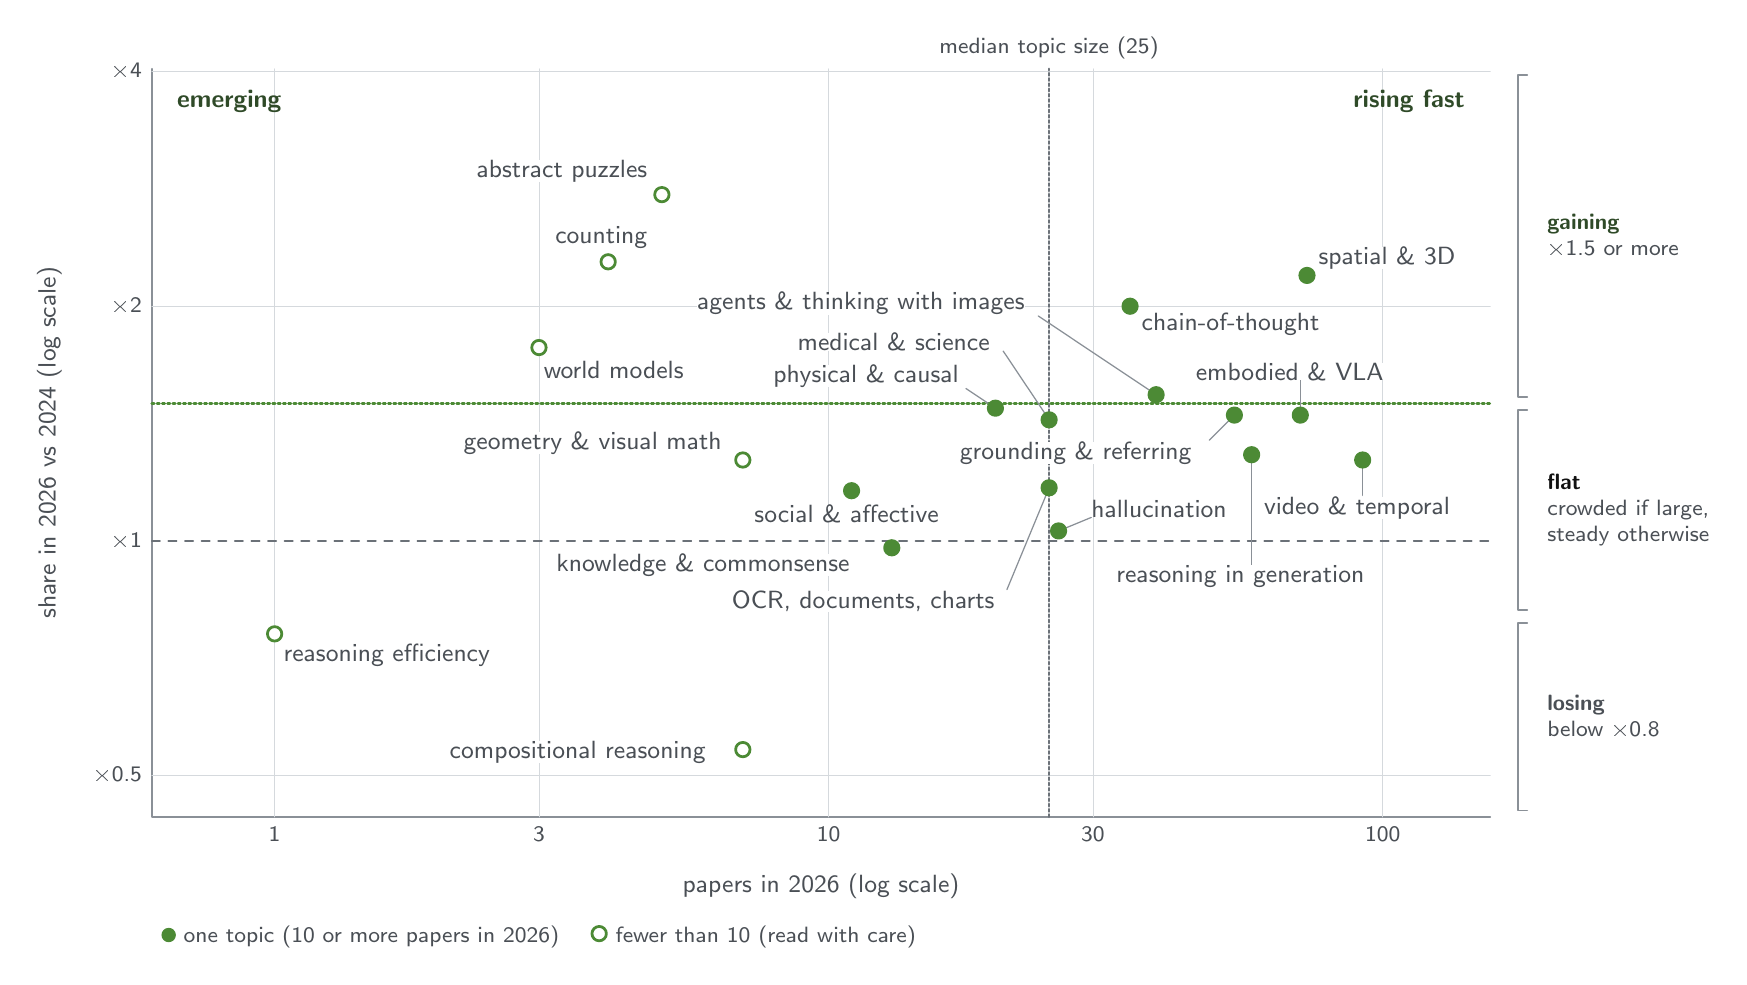
\begin{tikzpicture}[font=\small]
\draw[grey400, line width=0.6pt] (0,9.5) -- (0,0) -- (17.0,0);
\draw[grey300, line width=0.3pt] (1.561,0) -- (1.561,9.5); \node[below, font=\footnotesize, text=grey700] at (1.561,0) {1};
\draw[grey300, line width=0.3pt] (4.918,0) -- (4.918,9.5); \node[below, font=\footnotesize, text=grey700] at (4.918,0) {3};
\draw[grey300, line width=0.3pt] (8.597,0) -- (8.597,9.5); \node[below, font=\footnotesize, text=grey700] at (8.597,0) {10};
\draw[grey300, line width=0.3pt] (11.954,0) -- (11.954,9.5); \node[below, font=\footnotesize, text=grey700] at (11.954,0) {30};
\draw[grey300, line width=0.3pt] (15.633,0) -- (15.633,9.5); \node[below, font=\footnotesize, text=grey700] at (15.633,0) {100};
\draw[grey300, line width=0.3pt] (0,0.523) -- (17.0,0.523); \node[left, font=\footnotesize, text=grey700] at (0,0.523) {×0.5};
\draw[grey500, dashed, line width=0.6pt] (0,3.504) -- (17.0,3.504); \node[left, font=\footnotesize, text=grey700] at (0,3.504) {×1};
\draw[grey300, line width=0.3pt] (0,6.485) -- (17.0,6.485); \node[left, font=\footnotesize, text=grey700] at (0,6.485) {×2};
\draw[grey300, line width=0.3pt] (0,9.467) -- (17.0,9.467); \node[left, font=\footnotesize, text=grey700] at (0,9.467) {×4};
\draw[cvpr, densely dotted, line width=0.9pt] (0,5.248) -- (17.0,5.248);
\draw[grey500, densely dotted, line width=0.9pt] (11.397,0) -- (11.397,9.5);
\node[above, font=\footnotesize, text=grey700] at (11.397,9.5) {median topic size (25)};
\node[anchor=north west, font=\small\bfseries, text=ferndark] at (0.2,9.35) {emerging};
\node[anchor=north east, font=\small\bfseries, text=ferndark] at (16.8,9.35) {rising fast};
\draw[grey400, line width=0.6pt] (17.470000000000002,5.328) -- (17.35,5.328) -- (17.35,9.420) -- (17.470000000000002,9.420);
\node[anchor=west, align=left, font=\footnotesize, text=grey700] at (17.6,7.374) {\textbf{\color{ferndark}gaining}\\×1.5 or more};
\draw[grey400, line width=0.6pt] (17.470000000000002,2.624) -- (17.35,2.624) -- (17.35,5.168) -- (17.470000000000002,5.168);
\node[anchor=west, align=left, font=\footnotesize, text=grey700] at (17.6,3.896) {\textbf{\color{ink}flat}\\crowded if large,\\steady otherwise};
\draw[grey400, line width=0.6pt] (17.470000000000002,0.080) -- (17.35,0.080) -- (17.35,2.464) -- (17.470000000000002,2.464);
\node[anchor=west, align=left, font=\footnotesize, text=grey700] at (17.6,1.272) {\textbf{\color{grey700}losing}\\below ×0.8};
\node[below, font=\small, text=grey700] at (8.5,-0.6) {papers in 2026 (log scale)};
\node[rotate=90, font=\small, text=grey700] at (-1.3,4.75) {share in 2026 vs 2024 (log scale)};
\draw[grey400, line width=0.45pt] (13.680,5.031) -- (13.432,4.784);
\node[anchor=base west, inner sep=0pt, outer sep=0pt, fill=white, font=\small, text=grey700] at (10.264,4.541) {grounding \& referring};
\node[anchor=base west, inner sep=0pt, outer sep=0pt, fill=white, font=\small, text=grey700] at (5.125,7.282) {counting};
\draw[grey400, line width=0.45pt] (11.359,4.087) -- (10.861,2.886);
\node[anchor=base west, inner sep=0pt, outer sep=0pt, fill=white, font=\small, text=grey700] at (7.369,2.647) {OCR, documents, charts};
\draw[grey400, line width=0.45pt] (11.609,3.669) -- (11.933,3.803);
\node[anchor=base west, inner sep=0pt, outer sep=0pt, fill=white, font=\small, text=grey700] at (11.933,3.807) {hallucination};
\node[anchor=base west, inner sep=0pt, outer sep=0pt, fill=white, font=\small, text=grey700] at (14.819,7.013) {spatial \& 3D};
\node[anchor=base west, inner sep=0pt, outer sep=0pt, fill=white, font=\small, text=grey700] at (3.961,4.669) {geometry \& visual math};
\draw[grey400, line width=0.45pt] (15.379,4.432) -- (15.379,4.082);
\node[anchor=base west, inner sep=0pt, outer sep=0pt, fill=white, font=\small, text=grey700] at (14.127,3.843) {video \& temporal};
\draw[grey400, line width=0.45pt] (10.632,5.246) -- (10.341,5.440);
\node[anchor=base west, inner sep=0pt, outer sep=0pt, fill=white, font=\small, text=grey700] at (7.894,5.516) {physical \& causal};
\node[anchor=base west, inner sep=0pt, outer sep=0pt, fill=white, font=\small, text=grey700] at (4.979,5.573) {world models};
\node[anchor=base west, inner sep=0pt, outer sep=0pt, fill=white, font=\small, text=grey700] at (5.139,3.117) {knowledge \& commonsense};
\node[anchor=base west, inner sep=0pt, outer sep=0pt, fill=white, font=\small, text=grey700] at (7.655,3.743) {social \& affective};
\node[anchor=base west, inner sep=0pt, outer sep=0pt, fill=white, font=\small, text=grey700] at (4.125,8.126) {abstract puzzles};
\node[anchor=base west, inner sep=0pt, outer sep=0pt, fill=white, font=\small, text=grey700] at (3.785,0.741) {compositional reasoning};
\draw[grey400, line width=0.45pt] (14.587,5.202) -- (14.587,5.544);
\node[anchor=base west, inner sep=0pt, outer sep=0pt, fill=white, font=\small, text=grey700] at (13.260,5.547) {embodied \& VLA};
\draw[grey400, line width=0.45pt] (12.673,5.417) -- (11.259,6.361);
\node[anchor=base west, inner sep=0pt, outer sep=0pt, fill=white, font=\small, text=grey700] at (6.926,6.437) {agents \& thinking with images};
\node[anchor=base west, inner sep=0pt, outer sep=0pt, fill=white, font=\small, text=grey700] at (12.573,6.181) {chain-of-thought};
\node[anchor=base west, inner sep=0pt, outer sep=0pt, fill=white, font=\small, text=grey700] at (1.674,1.967) {reasoning efficiency};
\draw[grey400, line width=0.45pt] (13.969,4.499) -- (13.969,3.199);
\node[anchor=base west, inner sep=0pt, outer sep=0pt, fill=white, font=\small, text=grey700] at (12.251,2.979) {reasoning in generation};
\draw[grey400, line width=0.45pt] (11.342,5.126) -- (10.814,5.915);
\node[anchor=base west, inner sep=0pt, outer sep=0pt, fill=white, font=\small, text=grey700] at (8.204,5.919) {medical \& science};
\fill[cvpr, draw=cvpr, line width=1pt] (13.750,5.102) circle (2.6pt);
\fill[white, draw=cvpr, line width=1pt] (5.797,7.049) circle (2.6pt);
\fill[cvpr, draw=cvpr, line width=1pt] (11.397,4.179) circle (2.6pt);
\fill[cvpr, draw=cvpr, line width=1pt] (11.517,3.631) circle (2.6pt);
\fill[cvpr, draw=cvpr, line width=1pt] (14.672,6.876) circle (2.6pt);
\fill[white, draw=cvpr, line width=1pt] (7.507,4.532) circle (2.6pt);
\fill[cvpr, draw=cvpr, line width=1pt] (15.379,4.532) circle (2.6pt);
\fill[cvpr, draw=cvpr, line width=1pt] (10.715,5.190) circle (2.6pt);
\fill[white, draw=cvpr, line width=1pt] (4.918,5.960) circle (2.6pt);
\fill[cvpr, draw=cvpr, line width=1pt] (9.399,3.417) circle (2.6pt);
\fill[cvpr, draw=cvpr, line width=1pt] (8.888,4.142) circle (2.6pt);
\fill[white, draw=cvpr, line width=1pt] (6.479,7.902) circle (2.6pt);
\fill[white, draw=cvpr, line width=1pt] (7.507,0.854) circle (2.6pt);
\fill[cvpr, draw=cvpr, line width=1pt] (14.587,5.102) circle (2.6pt);
\fill[cvpr, draw=cvpr, line width=1pt] (12.756,5.361) circle (2.6pt);
\fill[cvpr, draw=cvpr, line width=1pt] (12.425,6.485) circle (2.6pt);
\fill[white, draw=cvpr, line width=1pt] (1.561,2.324) circle (2.6pt);
\fill[cvpr, draw=cvpr, line width=1pt] (13.969,4.599) circle (2.6pt);
\fill[cvpr, draw=cvpr, line width=1pt] (11.397,5.042) circle (2.6pt);
\node[anchor=north west, font=\footnotesize, text=grey700] at (0,-1.25) {\tikz\fill[cvpr] (0,0) circle (2.6pt); one topic (10 or more papers in 2026) \quad \tikz\draw[cvpr, fill=white, line width=1pt] (0,0) circle (2.6pt); fewer than 10 (read with care)};
\end{tikzpicture}
\end{document}
